\documentclass[10pt]{article}
\usepackage[margin=0.72in]{geometry}
\usepackage{graphicx,booktabs,hyperref}
\title{EKS image preflight for the n51 D5 stream trial}
\author{Semaev quotient-lift evidence packet}
\date{1 November 2026}
\begin{document}
\maketitle
\noindent The pinned EKS image completed one native small-system control. Its 1,040-byte D5 candidate was streamed to the assigned S3 prefix, fully read back, and accepted by the original checker with codimension 3. A separate host download reproduced SHA-256 \texttt{7cf2d46d96fe...e82d73}. This qualifies transport and checker behavior in the image; the n51 frontier result is separate.
\begin{center}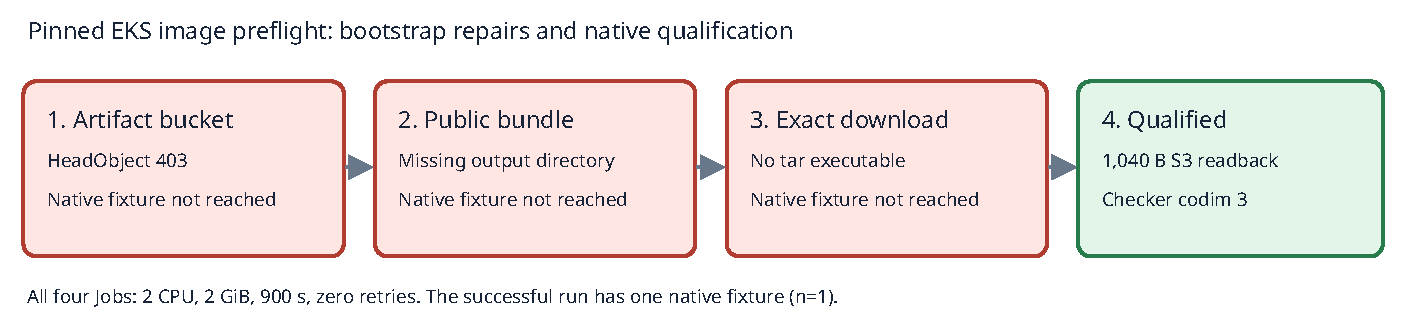
\includegraphics[width=\textwidth]{preflight-pipeline.pdf}\end{center}
\begin{center}\begin{tabular}{lll}\toprule
Attempt & Bootstrap or native result & Fixture reached?\\\midrule
Artifact-store source & S3 HeadObject 403 & No\\
Public source & Output directory absent & No\\
Public source v2 & No tar executable & No\\
Public source v3 & Full S3 readback; checker codimension 3 & Yes\\\bottomrule
\end{tabular}\end{center}
\noindent Successful Job: \texttt{semaev-d5-stream-custody-preflight-public-v3-20261101}.\\
Job UID: \texttt{ef4cb600-5b65-4ead-ba22-38f87369270b}. Image digest ends \texttt{0e4581}; limits: 2 CPU, 2 GiB, 900 seconds, zero retries. The exact 120,902-byte public bundle has SHA-256 \texttt{3be9cffdf5fb...7bfc103}. The adjacent \texttt{preflight/} directory contains the S3 readback manifest, original checker transcript, Job receipt, transfer result, and candidate bytes. Only the fourth Job reached the native fixture. No n51 degree-six claim follows from this control.
\end{document}
